% implementation structures O(1), Vertex, Triangle, Observables

% Store the geometry
% Naïve solution: use slice structure to store a sequence of up-down
% Performing moves meaning moving triangles, meaning O(N) complexity
% Solution: store list with connectivities
% Distances are of intrest so natural to look at connectivity of vertices
% Computationally simplier is to look at connectivity of triangles
% Finally: store an ordered list where every element represents a triangle, which stores the triangle indices it is connected to, and it's type (up-down)
% In this way both moves can be done in O(1), the 4-4 move without rejection and the 2-2 flip with rejection rate of approximately 50%

% To research data obtain 


\begin{frame}
    \frametitle{Observables}

    % To be able to analyse the behaviour of the model, meaningful observables need to be found
    \begin{itemize}
        \item Difficult to find meaningful observables
        \item Cannot depend on labeling $\rightarrow$ average over geometry
        \item ...
    \end{itemize}
    \begin{figure}
       \centering
       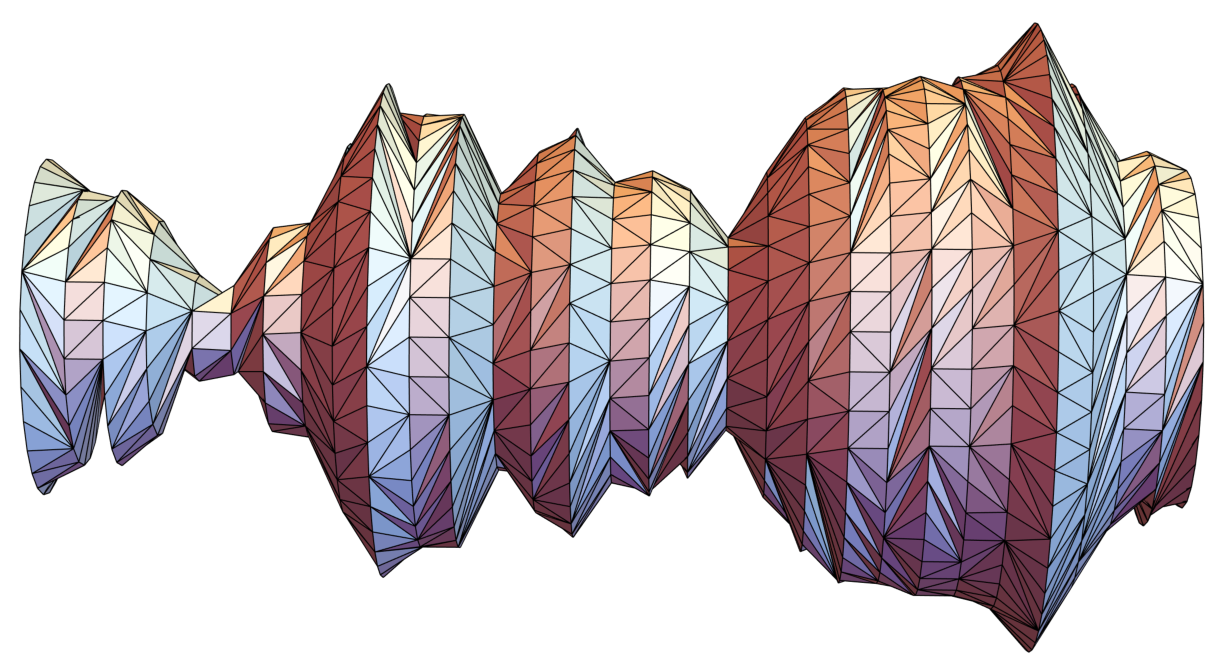
\includegraphics[width=0.6\linewidth]{img/triangulation.pdf}    
    \end{figure}

\end{frame}